%!TeX root = KraetkeZiegenhagen_CI.tex
\section{Jenkins -- Installation}

In diesem Abschnitt möchte ich kurz zeigen, wie man Jenkins installieren und konfigurieren muss, um eigene \LaTeX-Dokumente damit zu übersetzen.

Jenkins bildet die Softwarebasis, die wir zur Steuerung des Build-Prozesses nutzen werden und wurde ursprünglich unter dem Namen \enquote{Hudson} bei Sun Microsystems entwickelt. Jenkins benötigt Java -- es basiert auf den sogenannten \enquote{Enterprise Java Beans} und wird über den Webbrowser bedient. 

Im folgenden beschreibe ich das Setup unter Ubuntu, es sind aber auch Installationspakete für Windows, Mac OS X und diverse Linux-Varianten verfügbar.

Die eigentliche Installation verläuft unspektakulär, siehe das folgende Listing. Bei den meisten Debian-basierten Linuxen dürfte ein \lstinline{apt-get update} mit anschließendem \lstinline{apt-get install jenkins} ausreichen, für meine Linux-Version Xubuntu \enquote{Yakkety Yak} gab es jedoch noch kein Paket, sodass ich das Debian Repository einbinden musste, siehe \url{https://pkg.jenkins.io/debian/}.

\begin{lstlisting}{caption={jenkins Installation},label={lis:install}}
wget -q -O - https://pkg.jenkins.io/debian/jenkins.io.key | sudo apt-key add -
# deb https://pkg.jenkins.io/debian binary/ in 
# die Datei /etc/apt/sources.list mit aufnehmen
sudo apt-get update
sudo apt-get install jenkins
\end{lstlisting}

Nach der Installation -- ein Neustart ist nicht notwendig -- kann dann über Port 8080 des Installationsrechners auf die jenkins-Oberfläche zugegriffen werden. Im ersten Schritt müssen wir das Initial-Passwort aus einer Datei der jenkins-Installation kopieren, siehe Abbildung \ref{fig:initial}. Ein Hinweis noch dazu: Wer keine explizite Security benötigt, kann \lstinline{<useSecurity>true</useSecurity>} in der \texttt{/var/lib/jenkins/config.xml} auf \texttt{false} setzen.

\begin{figure}
\fbox{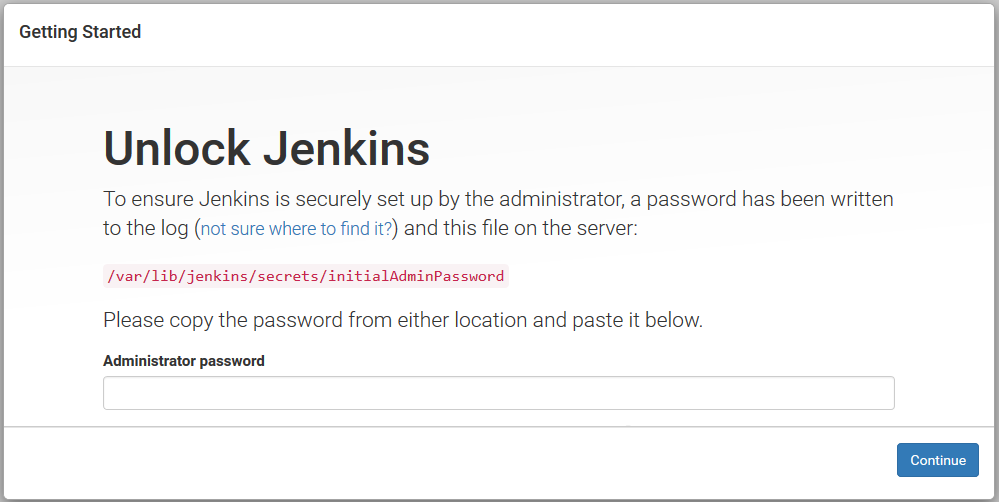
\includegraphics[width=\textwidth]{Images/Password}}
\caption{Festlegung des Initial-Passworts}\label{fig:initial}
\end{figure}

Im nächsten Schritt (siehe Abbildung \ref{fig:Plugins}) werden die Plugins ausgewählt, die wir benutzen möchten. Hier belasse ich es bei den Standard-Plugins, weitere lassen sich später nachinstallieren.

\begin{figure}
\fbox{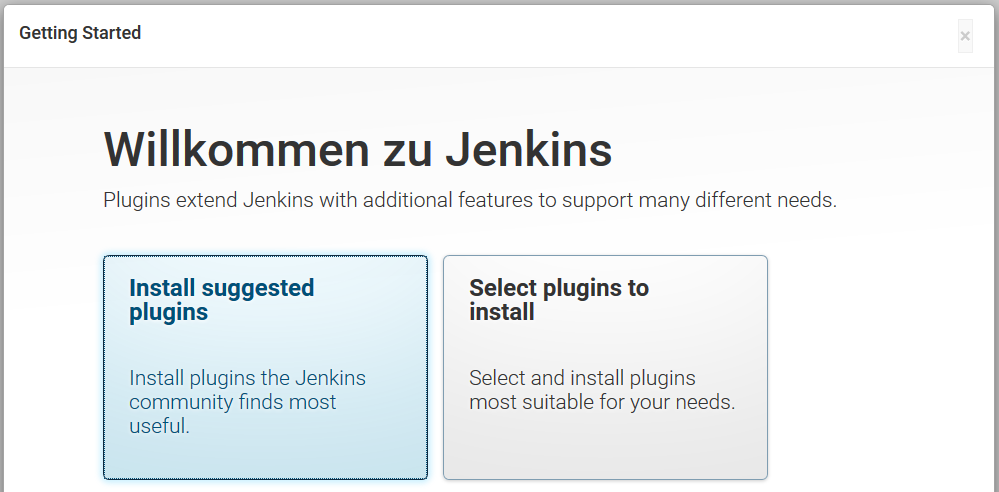
\includegraphics[width=\textwidth]{Images/Plugins}}
\caption{Auswahl der Plugins}\label{fig:Plugins}
\end{figure}


\begin{figure}
\fbox{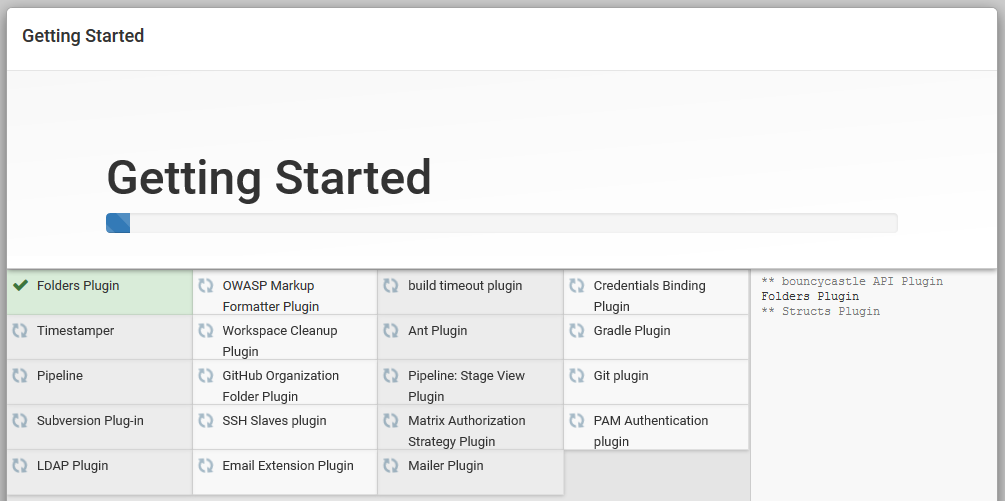
\includegraphics[width=\textwidth]{Images/Plugins2}}
\caption{Auswahl der Plugins}\label{fig:Plugins2}
\end{figure}

Nach der Erstellung eines Administratorkontos, siehe Abbildung \ref{fig:Admin}, können wir auf die Oberfläche zugreifen und neue Aufträge erstellen (siehe Abbildung \ref{fig:NewJob}).

\begin{figure}
\fbox{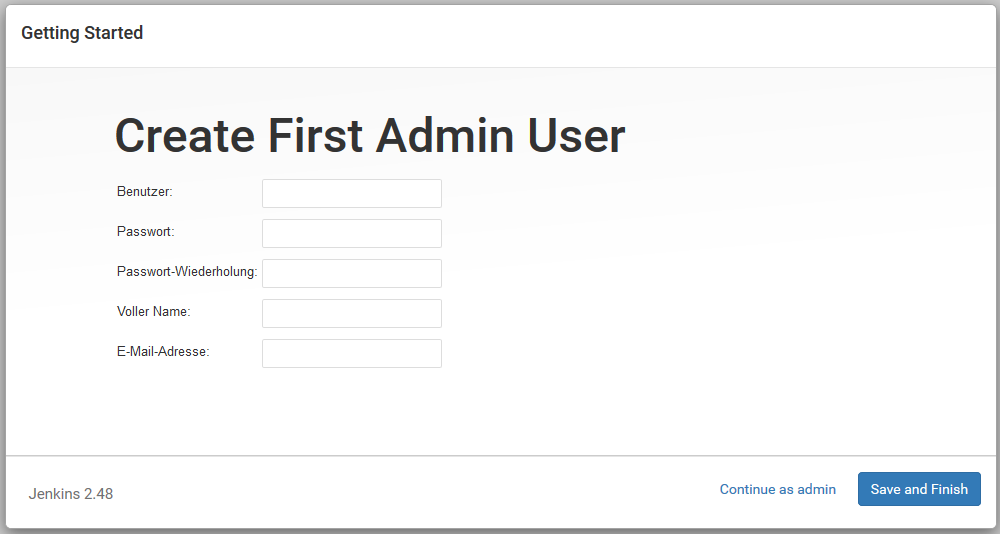
\includegraphics[width=\textwidth]{Images/Admin}}
\caption{Erstellung des Administrator-Kontos}\label{fig:Admin}
\end{figure}


\begin{figure}
\fbox{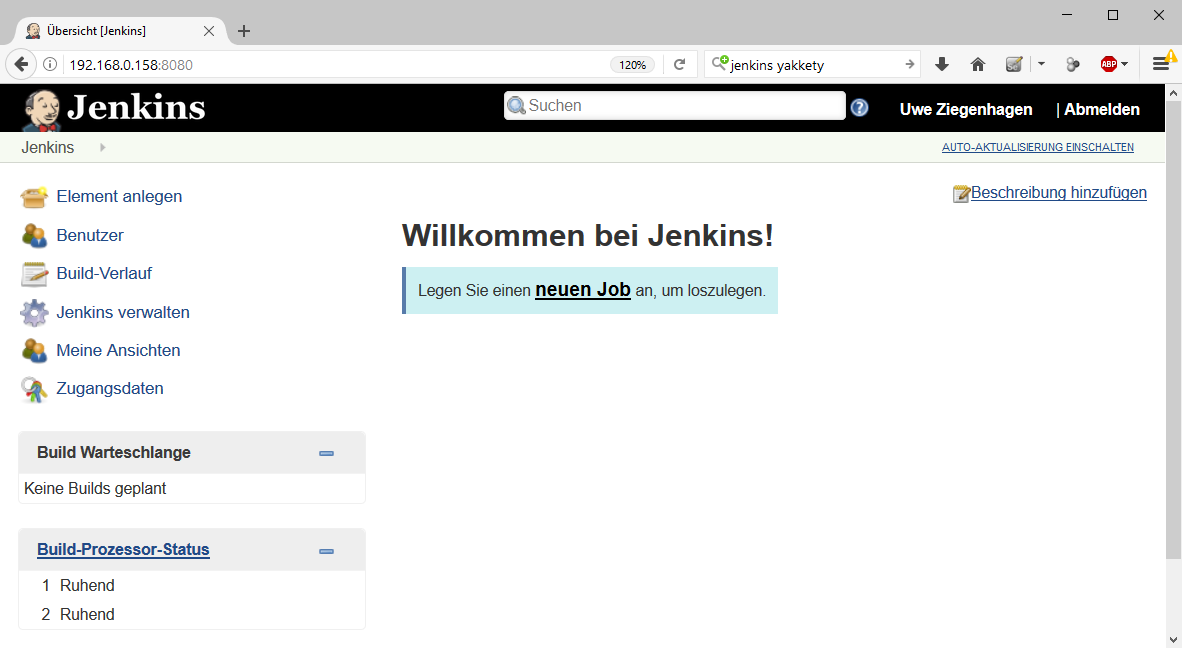
\includegraphics[width=\textwidth]{Images/NewJob}}
\caption{Die jenkins-Oberfläche}\label{fig:NewJob}
\end{figure}

\section{Jenkins in der praktischen Anwendung}

Angeregt durch eine Diskussion auf der internen Dante-Mailingliste hat sich in den letzten Monaten eine Gruppe Enthusiasten gefunden, die an einer Einführung zum Thema \enquote{\LaTeX\ für Geisteswissenschaftler} arbeitet. Aktuell sieben Mitstreiter haben sich zusammengetan, die verschiedene Themen bearbeiten. Die Zusammenarbeit wird über GitHub organisiert, auch die Projektdateien werden auf dieser Plattform (erreichbar unter \url{https://github.com/thomas-hilarius-meyer/LaTeX-fuer-Geisteswissenschaftler}) gespeichert. 

Bei der Zusammenarbeit hat sich gezeigt, dass Tippfehler bei der Eingabe oder unterschiedliche Versionsstände der \TeX-Installation dazu führten, dass das Gesamtprojekt nicht mehr kompilierbar war. 

Hier bietet sich Jenkins an, um die Kompilierung automatisch durchführen zu lassen. Als Hardware dient ein Intel NUC mit relativ schwachem Celeron N2820 und acht Gigabyte RAM, der unter Ubuntu-Linux läuft und über ein aktuelles \TeX\ Live 2016 verfügt.

In den allgemeinen Einstellungen, siehe Abbildung \ref{fig:jcommon}, legt man den Projektnamen fest sowie den Pfad zum GitHub-Projekt.

\begin{figure}
\fbox{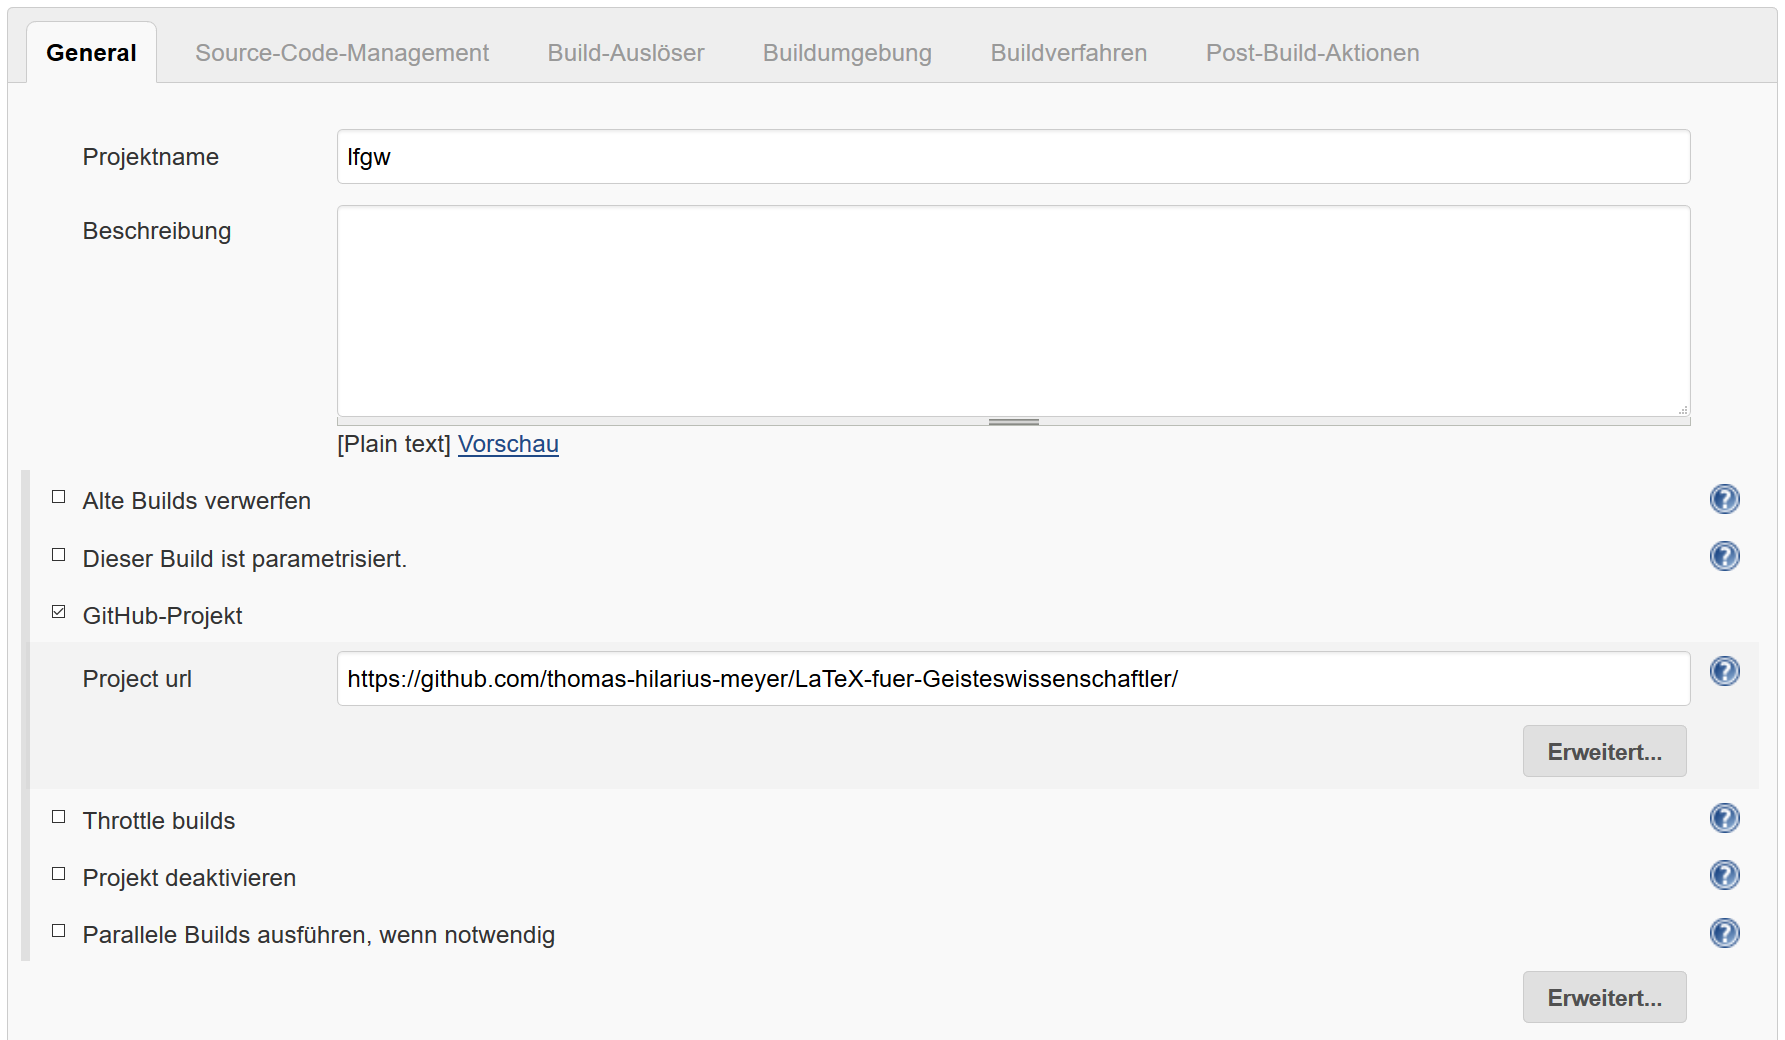
\includegraphics[width=\textwidth]{Images/lfgw-01}}
\caption{Allgemeine Einstellungen}\label{fig:jcommon}
\end{figure}

Unter \enquote{Source-Code-Management} (Abbildung \ref{fig:jgit}) wird dann nochmal der Zugang zum Projekt definiert, neben \texttt{git} unterstützt GitHub auch \texttt{Subversion} für den Zugriff auf die git-Repositories.


\begin{figure}
\fbox{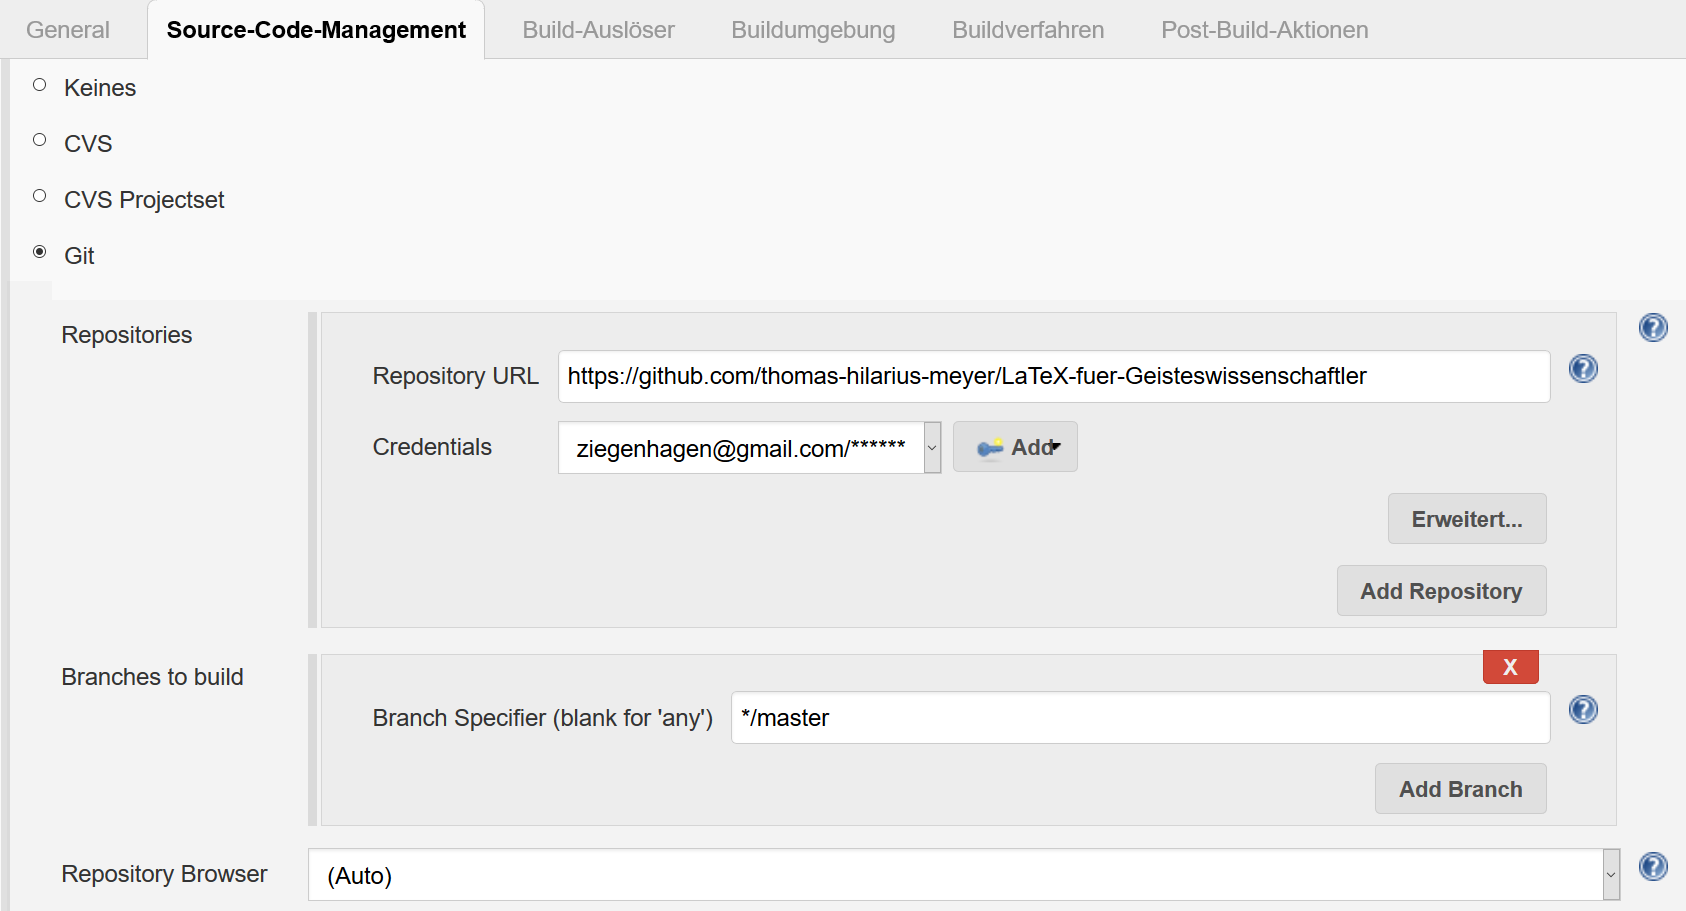
\includegraphics[width=\textwidth]{Images/lfgw-02}}
\caption{Zugang zum Repository}\label{fig:jgit}
\end{figure}

Um den Build-Job auszulösen gibt es verschiedene Möglichkeiten. Wir haben uns für das zeitgestützte Anstoßen entschieden (Details siehe Abbildung \ref{fig:jcron}), über eine \texttt{CRON} Syntax legen wir fest, dass täglich um Mitternacht der Build erfolgen soll. 


\begin{figure}
\fbox{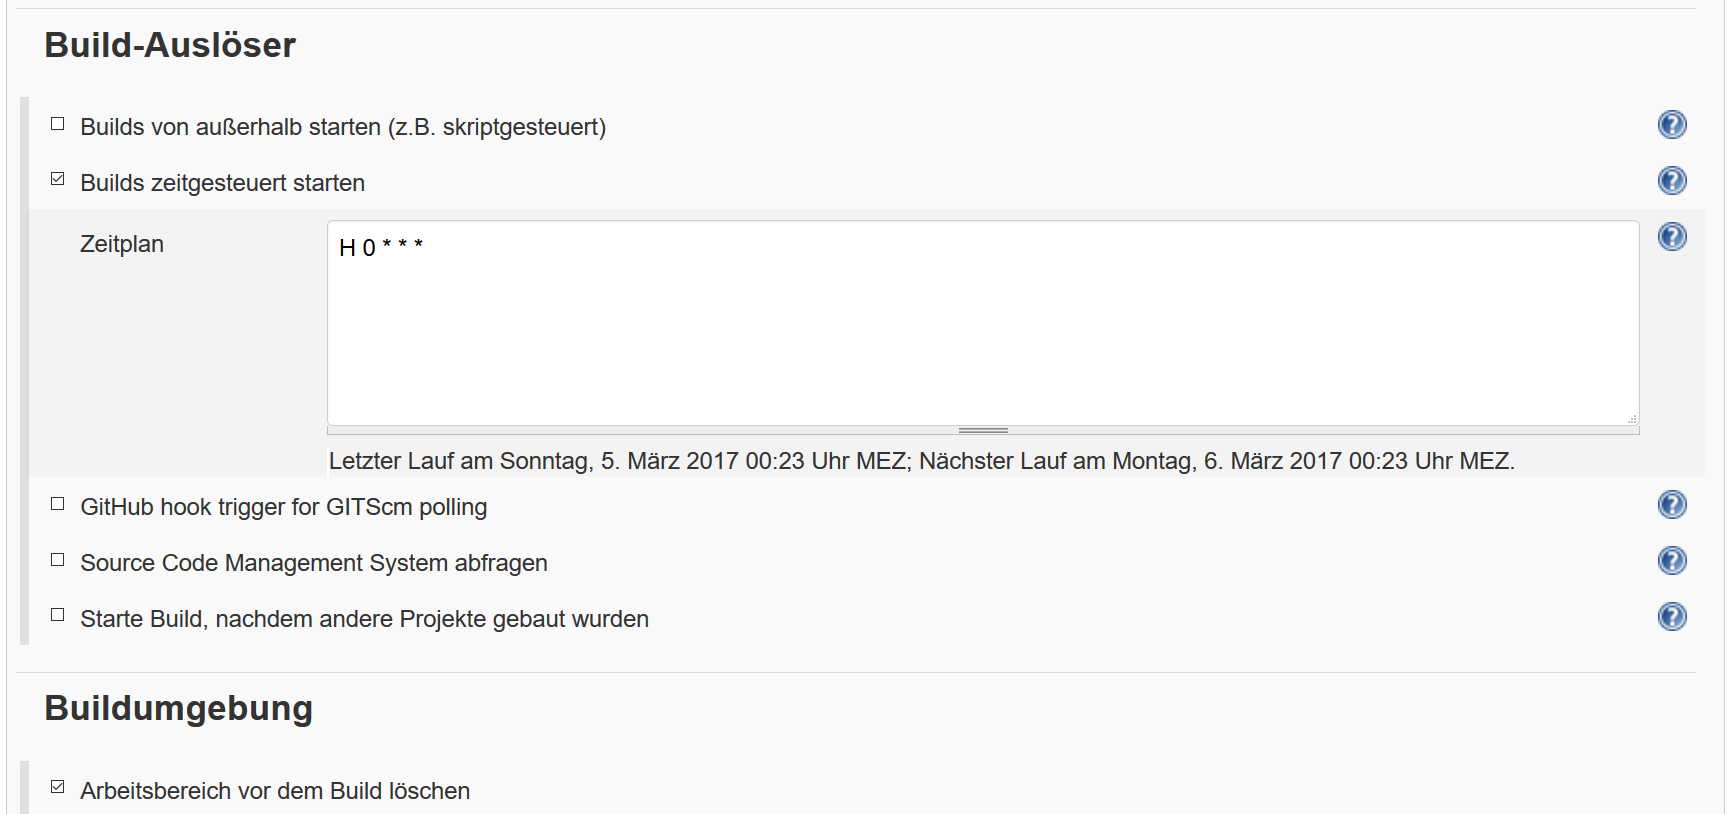
\includegraphics[width=\textwidth]{Images/lfgw-03}}
\caption{Zeitgesteuerte Auslösung}\label{fig:jcron}
\end{figure}


Unter \enquote{Buildverfahren} schließlich wird definiert, was für die Übersetzung geschehen muss, in unserem Fall lua\LaTeX\ gefolgt von \texttt{biber} und anschließendem erneuten lua\LaTeX. Alle drei Aufrufe schreiben ihre Ergebnisse in ein separates Verzeichnis, um nicht Probleme mit den Kompilierungen der einzelnen Co-Autorinnen und -Autoren zu verursachen. Abbildung \ref{fig:jcompile} zeigt die entsprechenden Aufrufe.


\begin{figure}
\fbox{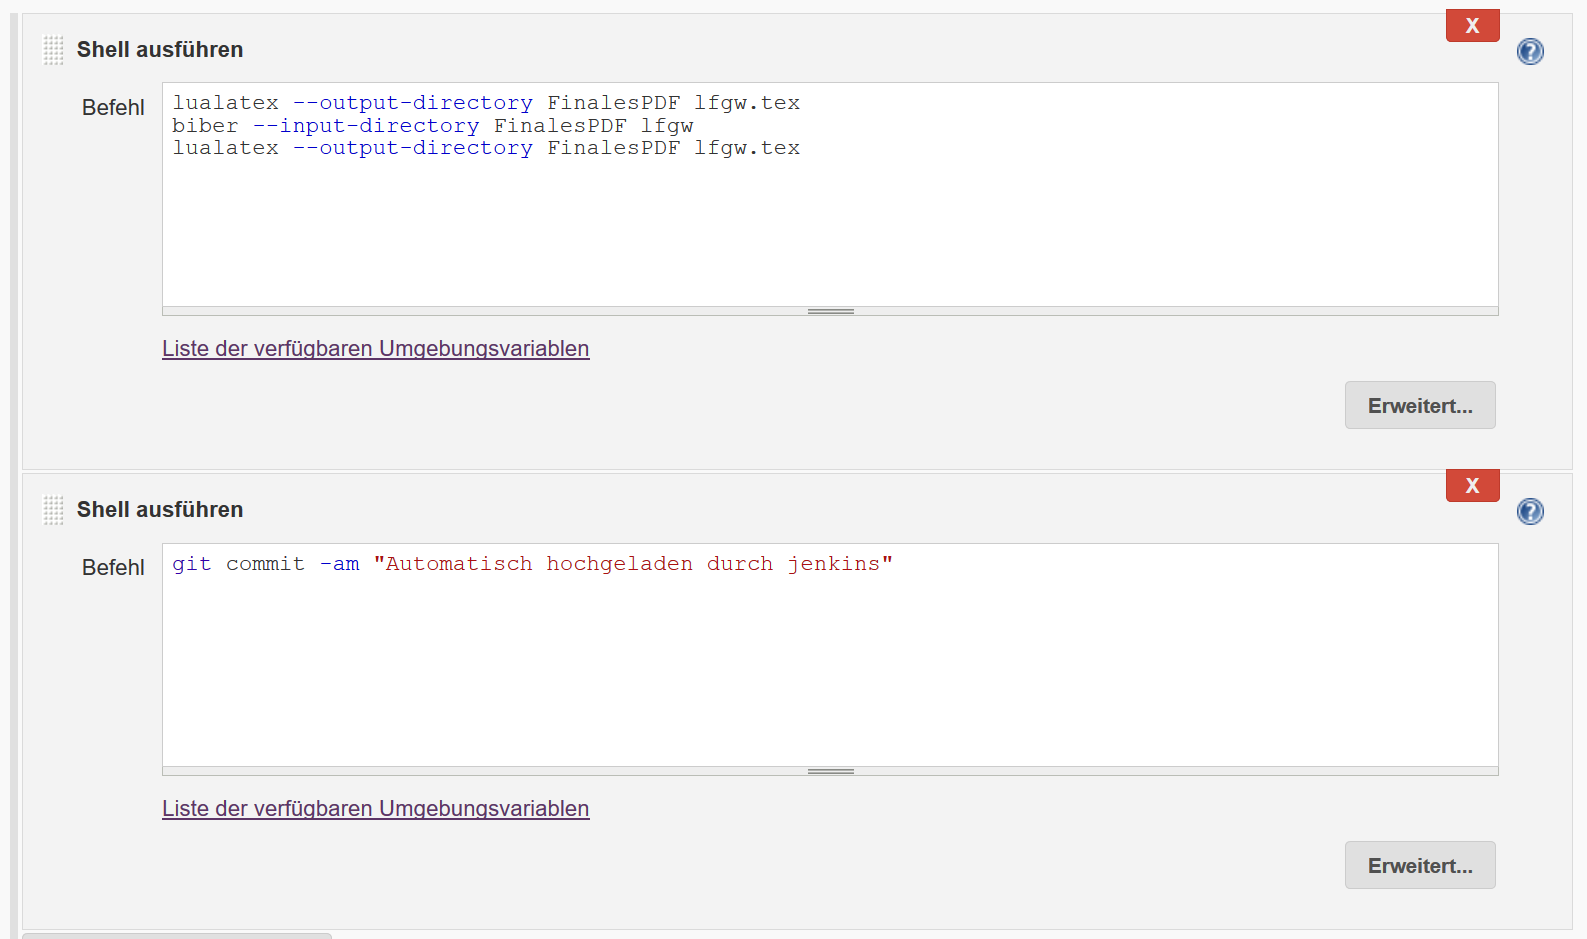
\includegraphics[width=\textwidth]{Images/lfgw-04}}
\caption{Die eigentliche Übersetzung}\label{fig:jcompile}
\end{figure}


Im Anschluss daran werden über den \texttt{git commit} Befehl die Änderungen (nur am PDF, da die \TeX-Dateien hier nicht verändert werden) in das Repository geschrieben.

Der finale Schritt (siehe Abbildung \ref{fig:backGitHub}) besteht dann darin, das geänderte PDF wieder zurück nach GitHub zu spielen.

\begin{figure}
\fbox{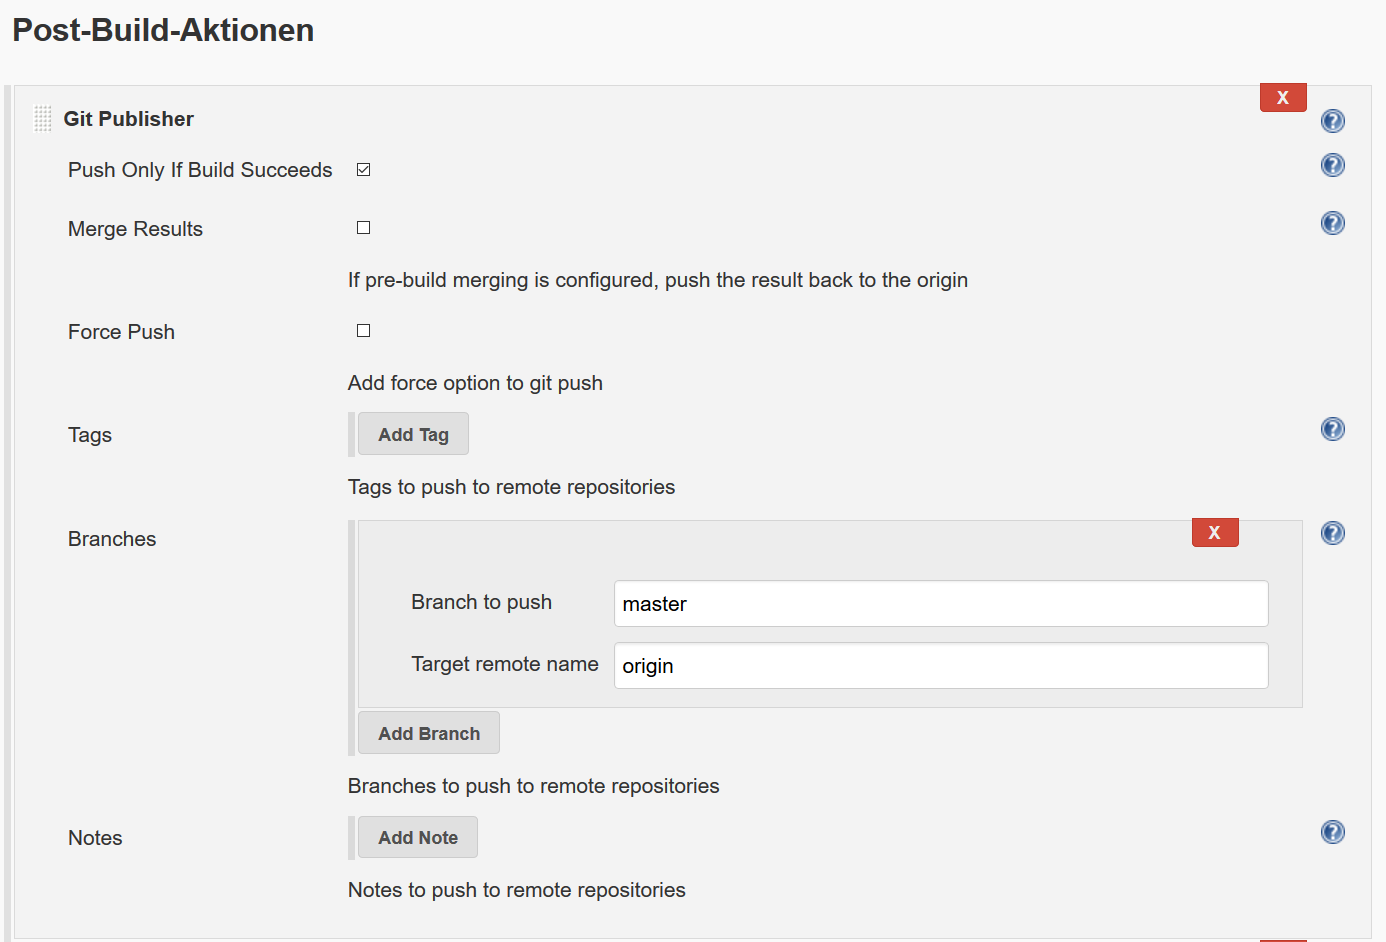
\includegraphics[width=\textwidth]{Images/lfgw-05}}
\caption{Der Weg zurück zu GitHub}\label{fig:backGitHub}
\end{figure}